\documentclass[../DoAn.tex]{subfiles}
\begin{document}

Chương này trình bày chi tiết các giải pháp kỹ thuật, kiến trúc tối ưu hóa hệ thống và những đóng góp nổi bật nhất trong suốt quá trình xây dựng dự án ``JobBridge AI''. Đây là những đóng góp khoa học và thực tiễn cốt lõi được tác giả tự tay nghiên cứu, thiết kế và triển khai nhằm giải quyết triệt để các vấn đề phức tạp về độ trễ AI, kỹ nghệ Prompt thích ứng, kiểm soát phân quyền microservices và tối ưu quy trình DevOps/Observability trên nền tảng đám mây.

\section{Giải pháp tối ưu hóa độ trễ xử lý dữ liệu với cơ chế Trích xuất và Cache văn bản CV từ tệp PDF}
\label{sec:solution-caching}

\subsection{Dẫn dắt và bài toán}
Trong các hệ thống tuyển dụng tích hợp Trí tuệ nhân tạo (AI), việc gửi toàn bộ tài liệu hồ sơ (CV) dạng tệp PDF gốc lên các mô hình ngôn ngữ lớn (LLM) mỗi khi thực hiện các yêu cầu (như chấm điểm CV hoặc phỏng vấn giả lập) gặp phải ba hạn chế chí mạng:
\begin{enumerate}
    \item \textbf{Độ trễ truyền tải lớn (Network Latency):} Việc tải tệp PDF nhị phân từ CDN (Cloudinary) về backend, sau đó truyền tiếp dữ liệu thô này hoặc nội dung văn bản chưa tối ưu sang OpenAI API gây tốn kém thời gian băng thông.
    \item \textbf{Quá tải Token và Chi phí:} Định dạng PDF chứa nhiều mã nhị phân bố cục và siêu dữ liệu không cần thiết cho AI. Việc đẩy trực tiếp tệp hoặc trích xuất động mỗi lần request làm tăng lượng token tiêu thụ đầu vào, tăng chi phí vận hành OpenAI API lên gấp nhiều lần.
    \item \textbf{Tắc nghẽn CPU ở Backend (Parsing Bottleneck):} Việc trích xuất văn bản từ tệp PDF bằng thư viện runtime mỗi khi có API request sẽ chiếm dụng tài nguyên CPU cực lớn của microservice, làm giảm thông lượng (Throughput) tổng thể của service đó khi có nhiều người dùng đồng thời.
\end{enumerate}

\subsection{Giải pháp thiết kế chi tiết}
Để giải quyết triệt để vấn đề này, tác giả đã thiết kế luồng xử lý dữ liệu CV theo cơ chế **Trích xuất một lần và Lưu bộ nhớ đệm chủ động (Extract-Once and Active Caching Flow)**. Luồng nghiệp vụ được thiết kế tối ưu như mô tả trong Hình \ref{fig:flow-cv-caching}.

\begin{figure}[H]
    \centering
    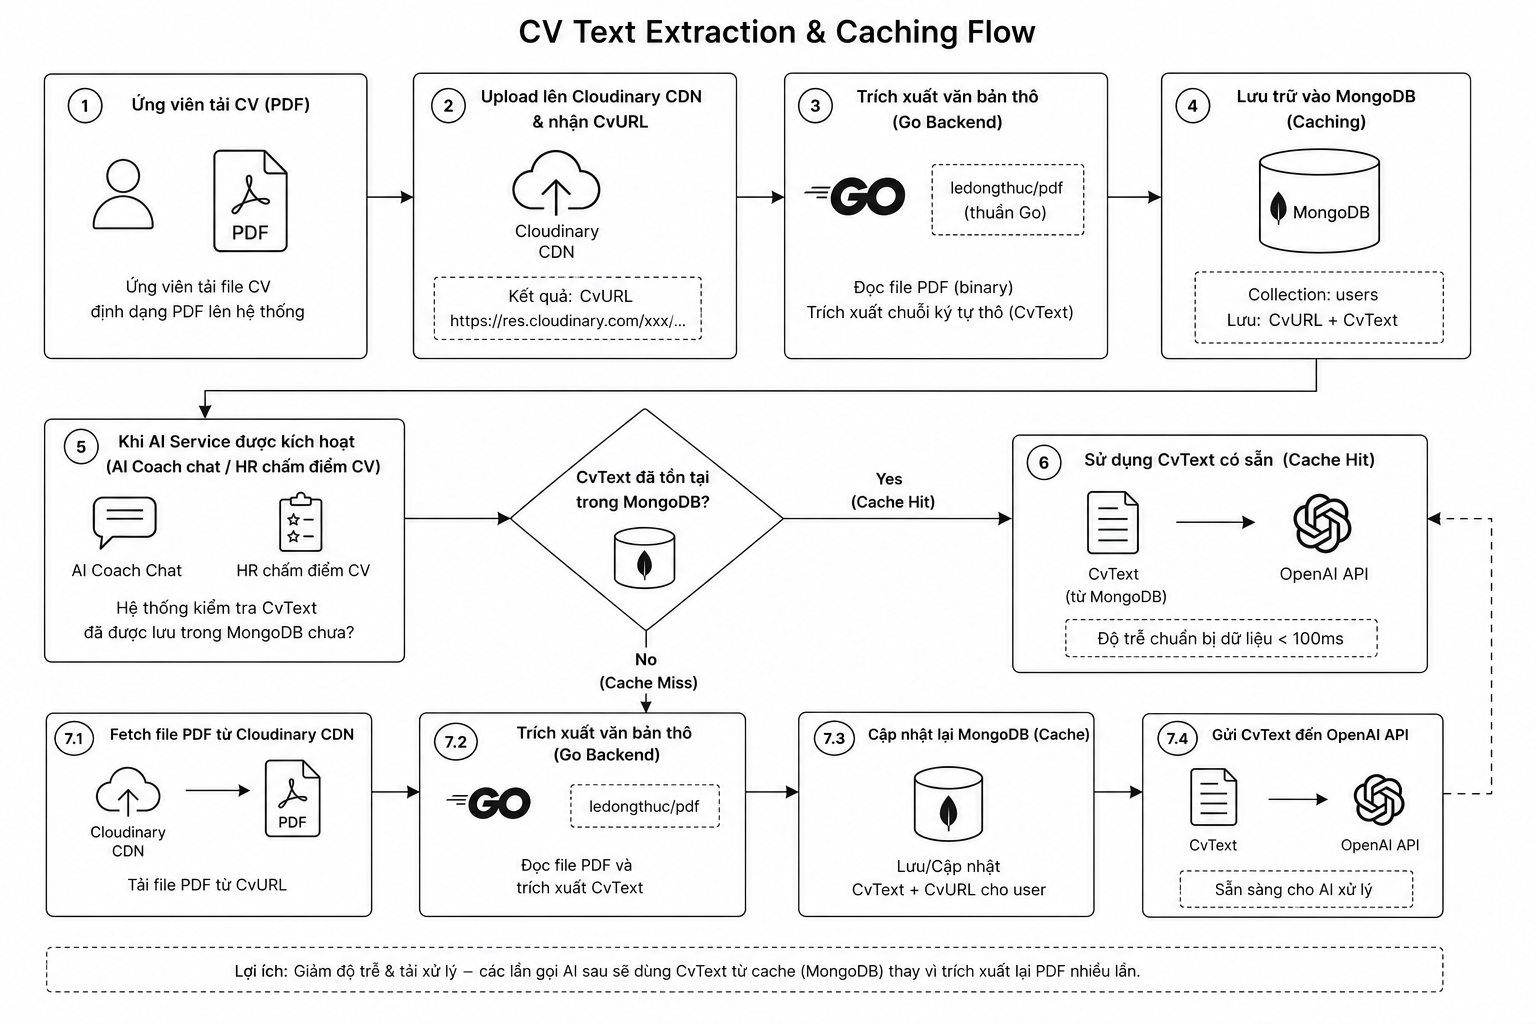
\includegraphics[width=0.9\textwidth]{so-do-chuong-5/flow_cv_extraction_caching.png}
    \caption{Sơ đồ luồng trích xuất văn bản và lưu bộ nhớ đệm (Cache) CV ứng viên.}
    \label{fig:flow-cv-caching}
\end{figure}

Giải pháp gồm các bước thực thi chi tiết sau:
\begin{itemize}
    \item \textbf{Bước 1: Trích xuất bất đồng bộ ngay khi cập nhật:} Khi ứng viên tải lên file PDF CV mới, Auth Service sẽ thực hiện lưu file gốc lên Cloudinary và lấy về URL. Ngay lập tức, một tiến trình Go thuần sử dụng thư viện hiệu năng cao \texttt{ledongthuc/pdf} để phân tích nhị phân và trích xuất chuỗi văn bản thuần túy (Raw Text), loại bỏ toàn bộ định dạng nhị phân rác.
    \item \textbf{Bước 2: Cache trực tiếp vào CSDL:} Chuỗi văn bản thô sau khi trích xuất được lưu trữ trực tiếp vào trường \texttt{cv\_text} thuộc collection \texttt{users} trong MongoDB.
    \item \textbf{Bước 3: Cơ chế Cache Lookup (Kiểm tra cache chủ động):} Khi các tính năng AI (AI Interview Coach hoặc AI Evaluate CV) được kích hoạt, AI Service sẽ kiểm tra trường \texttt{cv\_text} của ứng viên trong MongoDB trước:
    \begin{itemize}
        \item \textbf{Trường hợp Cache Hit (Trúng cache):} Lấy trực tiếp chuỗi văn bản thô đã lưu trong CSDL để gửi sang OpenAI API. Bỏ qua hoàn toàn bước tải file và trích xuất PDF.
        \item \textbf{Trường hợp Cache Miss (Trượt cache - dự phòng lỗi):} Hệ thống sẽ tải tệp PDF từ Cloudinary CDN, tiến hành trích xuất thô, cập nhật ngược lại MongoDB để làm cache cho các lần sau, rồi mới gửi dữ liệu đến OpenAI API.
    \end{itemize}
\end{itemize}

Quy trình giải thuật trích xuất văn bản thô từ luồng nhị phân (Binary stream parsing) của tệp PDF được hệ thống thực hiện tuần tự qua các pha xử lý nghiêm ngặt sau:
\begin{enumerate}
    \item \textbf{Pha 1 (Tải và Đệm dữ liệu):} Thực hiện yêu cầu HTTP GET bất đồng bộ tới URL lưu trữ của Cloudinary CDN. Luồng dữ liệu (Data stream) được đọc trực tiếp vào bộ đệm bộ nhớ RAM thông qua kiểu đối tượng \texttt{io.Reader} để tránh ghi ra đĩa cứng (Disk I/O), tối ưu hóa tốc độ đọc.
    \item \textbf{Pha 2 (Định dạng nhị phân):} Khởi tạo thực thể đọc PDF nhị phân \texttt{pdf.Reader} với kích thước được định lượng chính xác bằng độ dài byte thực tế của tệp tin.
    \item \textbf{Pha 3 (Giải mã văn bản):} Kích hoạt hàm chuyển đổi dữ liệu phẳng \texttt{GetPlainText()}, thực hiện quét qua toàn bộ cấu trúc các trang (Pages) của tệp tin PDF, lọc bỏ toàn bộ các thẻ nhị phân biểu diễn bố cục đồ họa, chỉ giữ lại các ký tự dạng chuỗi phẳng (Plain string).
    \item \textbf{Pha 4 (Lưu đệm):} Gom dữ liệu phẳng từ bộ đệm \texttt{bytes.Buffer} và chuyển đổi thành một chuỗi văn bản sạch (Cleaned string), sẵn sàng lưu trữ vào MongoDB.
\end{enumerate}

\subsection{Kết quả đạt được}
Giải pháp tích cực này mang lại các kết quả vượt trội về mặt kỹ thuật:
\begin{itemize}
    \item \textbf{Rút ngắn độ trễ vượt bậc:} Thời gian chuẩn bị dữ liệu đầu vào cho AI giảm từ $1.5$ giây (khi phải download và parse tệp PDF động) xuống còn dưới $20$ mili-giây (lấy chuỗi text trực tiếp từ MongoDB).
    \item \textbf{Giảm tải CPU Server:} CPU của cụm microservices không còn bị quá tải (CPU spikes) khi có nhiều yêu cầu phỏng vấn hoặc đánh giá diễn ra đồng thời, tăng đáng kể năng lực phục vụ đồng thời của hệ thống.
    \item \textbf{Tối ưu hóa băng thông:} Hệ thống không cần truyền tải tệp nhị phân giữa các thành phần nội bộ trong mạng AKS, giúp tiết kiệm băng thông hạ tầng cloud và giảm chi phí vận hành mạng trên Azure.
\end{itemize}

---

\section{Kỹ nghệ Prompt phân tầng thích ứng ngữ cảnh cho hệ thống phỏng vấn giả lập và đánh giá ứng viên}
\label{sec:solution-prompt}

\subsection{Dẫn dắt và bài toán}
Việc xây dựng một trợ lý phỏng vấn (AI Coach) hoặc hệ thống chấm điểm CV đòi hỏi tính chính xác, thực tế và khách quan cao. Các mô hình ngôn ngữ lớn (như GPT-4o-mini) nếu chỉ nhận được một Prompt chung chung rất dễ dẫn tới hiện tượng **ảo tưởng (hallucination)**:
\begin{itemize}
    \item AI đưa ra các câu hỏi phỏng vấn không khớp với mô tả công việc (JD) thực tế của doanh nghiệp.
    \item AI đánh giá hoặc đặt câu hỏi về những công nghệ mà ứng viên hoàn toàn không có kinh nghiệm trong CV (gây ức chế cho người dùng).
    \item AI bị mất dấu ngữ cảnh (Context drift) khi cuộc trò chuyện kéo dài, dẫn đến việc lặp lại câu hỏi hoặc trả lời lạc đề.
    \item Trả về định dạng văn bản hỗn độn, khó phân tách để hiển thị giao diện.
\end{itemize}

\subsection{Giải pháp thiết kế chi tiết}
Để giải quyết bài toán này, tác giả đã thiết kế **Kiến trúc Prompt Phân tầng Thích ứng Ngữ cảnh (Layered Context-Aware Prompt Architecture)**. Sơ đồ khối kiến trúc prompt được mô tả trong Hình \ref{fig:prompt-layered}.

\begin{figure}[H]
    \centering
    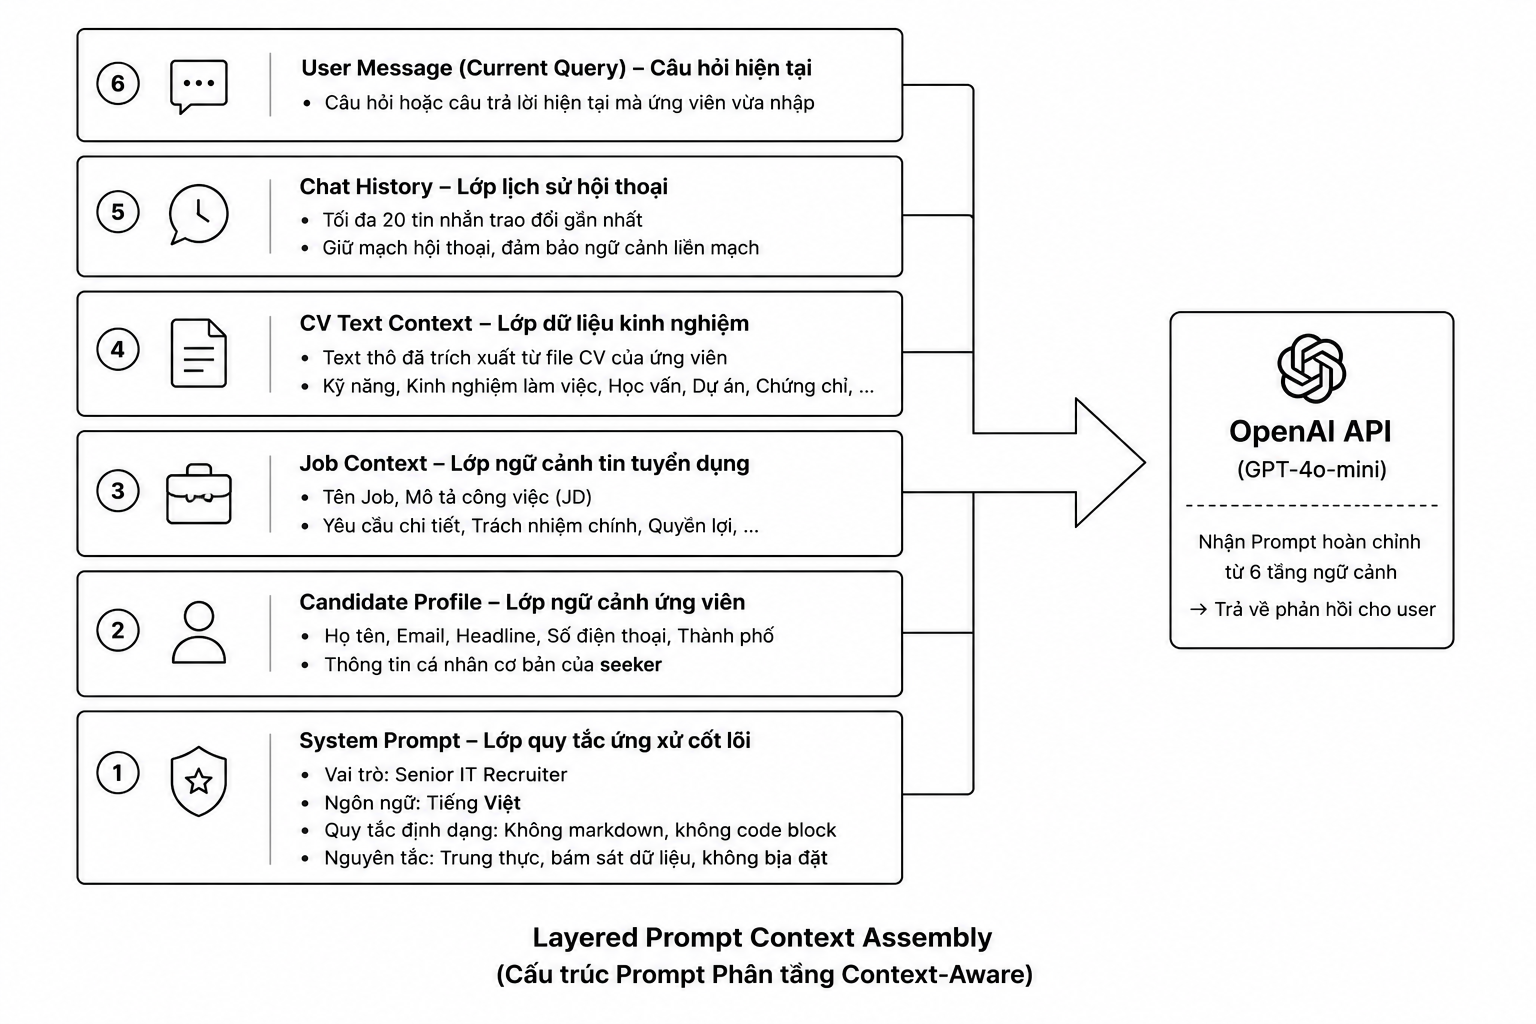
\includegraphics[width=0.9\textwidth]{so-do-chuong-5/prompt_layered_structure.png}
    \caption{Cấu trúc Prompt phân tầng lắp ghép ngữ cảnh động gửi tới OpenAI API.}
    \label{fig:prompt-layered}
\end{figure}

Khối prompt gửi đi được tự động lắp ghép bởi AI Service từ 6 tầng thông tin riêng biệt:
\begin{enumerate}
    \item \textbf{Tầng 1 (System Prompt - Quy tắc lõi):} Thiết lập vai trò cố định cho AI là chuyên gia tuyển dụng công nghệ cao cấp. Ràng buộc ngôn ngữ bắt buộc phải là tiếng Việt, giọng điệu chuyên nghiệp, xây dựng tính xây dựng. Đồng thời ép buộc cấu hình đầu ra (Output format) nghiêm ngặt để frontend dễ phân tích.
    \item \textbf{Tầng 2 (Candidate Profile - Ngữ cảnh ứng viên):} Tiêm các thông tin cơ bản của ứng viên (họ tên, mục tiêu nghề nghiệp) nhằm giúp AI xưng hô chính xác và cá nhân hóa hội thoại.
    \item \textbf{Tầng 3 (Job Context - Ngữ cảnh JD):} Trích xuất trực tiếp thông tin tuyển dụng từ CSDL (tên vị trí, yêu cầu kỹ thuật, trách nhiệm chính) để AI bám sát các tiêu chí tuyển dụng cốt lõi của công ty.
    \item \textbf{Tầng 4 (CV Text Context - Hồ sơ kinh nghiệm):} Trích xuất chuỗi văn bản CV thô đã được cache ở MongoDB. Lớp này giúp AI chỉ tập trung đào sâu vào các dự án, công nghệ mà ứng viên thực sự đã làm, tránh hỏi lan man các kiến thức ngoài tầm.
    \item \textbf{Tầng 5 (Chat History - Bộ nhớ đệm giới hạn):} Lưu trữ tối đa 20 tin nhắn trò chuyện gần nhất theo cấu trúc hàng đợi (FIFO). Cơ chế giới hạn này vừa duy trì được ngữ cảnh liên tục của buổi phỏng vấn, vừa tránh hiện tượng tràn cửa sổ ngữ cảnh (Context Window) gây tăng chi phí token.
    \item \textbf{Tầng 6 (User Message):} Câu trả lời hiện tại của ứng viên để AI tiếp tục đánh giá và đặt câu hỏi tiếp theo.
\end{enumerate}

Về mặt lý thuyết cấu trúc thông tin, Prompt phân tầng được xây dựng dưới dạng một hàm số tổng hợp ngữ cảnh động $F(C)$, trong đó ngữ cảnh gửi đến LLM được biểu diễn bằng một tập hợp có thứ tự các phân lớp thông tin:
\begin{equation}
    C_{prompt} = \{S, P, J, V, H_{k}, M_{user}\}
\end{equation}
Trong đó các thành phần được định nghĩa cụ thể:
\begin{itemize}
    \item $S$ (System Instruction): Các quy tắc ràng buộc cốt lõi và định dạng đầu ra bắt buộc của AI.
    \item $P$ (Profile): Thông tin định danh của ứng viên thực hiện phỏng vấn.
    \item $J$ (Job Description): Ngữ cảnh mô tả công việc và các tiêu chí tuyển dụng.
    \item $V$ (Volume of CV): Văn bản CV đã qua trích xuất sạch và cache trong CSDL.
    \item $H_{k}$ (History): Chuỗi hội thoại lịch sử có chặn giới hạn $k$ tin nhắn gần nhất ($k \le 20$).
    \item $M_{user}$ (Message): Câu trả lời hiện tại của ứng viên gửi lên hệ thống.
\end{itemize}

Cơ chế này đảm bảo rằng mỗi khi có tin nhắn mới từ người dùng, hệ thống sẽ thực hiện truy vấn và lắp ghép các lớp thông tin này thành một mảng cấu trúc tin nhắn động có định dạng JSON chuẩn gửi trực tiếp đến OpenAI API mà không bị dư thừa token rác.

\subsection{Kết quả đạt được}
\begin{itemize}
    \item \textbf{Triệt tiêu hiện tượng ảo tưởng:} Loại bỏ hoàn toàn tình trạng AI đặt câu hỏi nằm ngoài phạm vi kỹ năng của ứng viên hoặc JD công việc.
    \item \textbf{Cá nhân hóa cao:} Trải nghiệm người dùng cực kỳ chân thực, AI tương tác tự nhiên, thông minh như một nhà tuyển dụng có chuyên môn cao đang trực tiếp đối thoại.
    \item \textbf{Độ tin cậy của dữ liệu đầu ra:} Cấu trúc phản hồi luôn tuân thủ nghiêm ngặt định dạng hiển thị, loại bỏ hoàn toàn các lỗi hiển thị giao diện ở phía client.
\end{itemize}

---

\section{Giải pháp bảo mật phân lớp và kiểm soát tài nguyên nghiệp vụ tại API Gateway và Microservices}
\label{sec:solution-security}

\subsection{Dẫn dắt và bài toán}
Trong một hệ thống phân tán gồm nhiều Microservices giao tiếp qua lại, việc chỉ bảo vệ xác thực (Authentication) tại API Gateway bằng cách giải mã Token JWT là chưa đủ để đảm bảo tính an toàn cho tài nguyên nghiệp vụ (Business Authorization):
\begin{itemize}
    \item \textbf{Nguy cơ bỏ qua kiểm tra quyền (Authorization Bypass):} Một kẻ tấn công có tài khoản ứng viên hợp lệ (có Token JWT đúng cấu trúc) có thể cố tình gọi trực tiếp vào API của Nhà tuyển dụng hoặc gọi các endpoint chấm điểm CV của AI để phá hoại nếu hệ thống chỉ kiểm tra tính hợp lệ của Token mà không kiểm tra quyền hạn thực tế (Role).
    \item \textbf{Tấn công giả mạo chủ sở hữu tài nguyên (ID Spoofing / Broken Object Level Authorization - BOLA):} Ứng viên A có thể cố tình thay đổi tham số \texttt{job\_id} trên API phỏng vấn sang một job B mà họ chưa từng ứng tuyển để đánh lừa hệ thống. Tương tự, Nhà tuyển dụng X có thể gửi yêu cầu AI chấm điểm CV của ứng viên ứng tuyển vào công ty Y (đối thủ cạnh tranh).
\end{itemize}

\subsection{Giải pháp thiết kế chi tiết}
Để loại bỏ hoàn toàn các lỗ hổng bảo mật nghiêm trọng này, tác giả đã triển khai **Giải pháp Bảo mật và Phân quyền Phân lớp (Layered Security Authorization Architecture)** bao gồm 3 lớp bảo vệ chặt chẽ như mô tả ở Hình \ref{fig:security-layered}.

\begin{figure}[H]
    \centering
    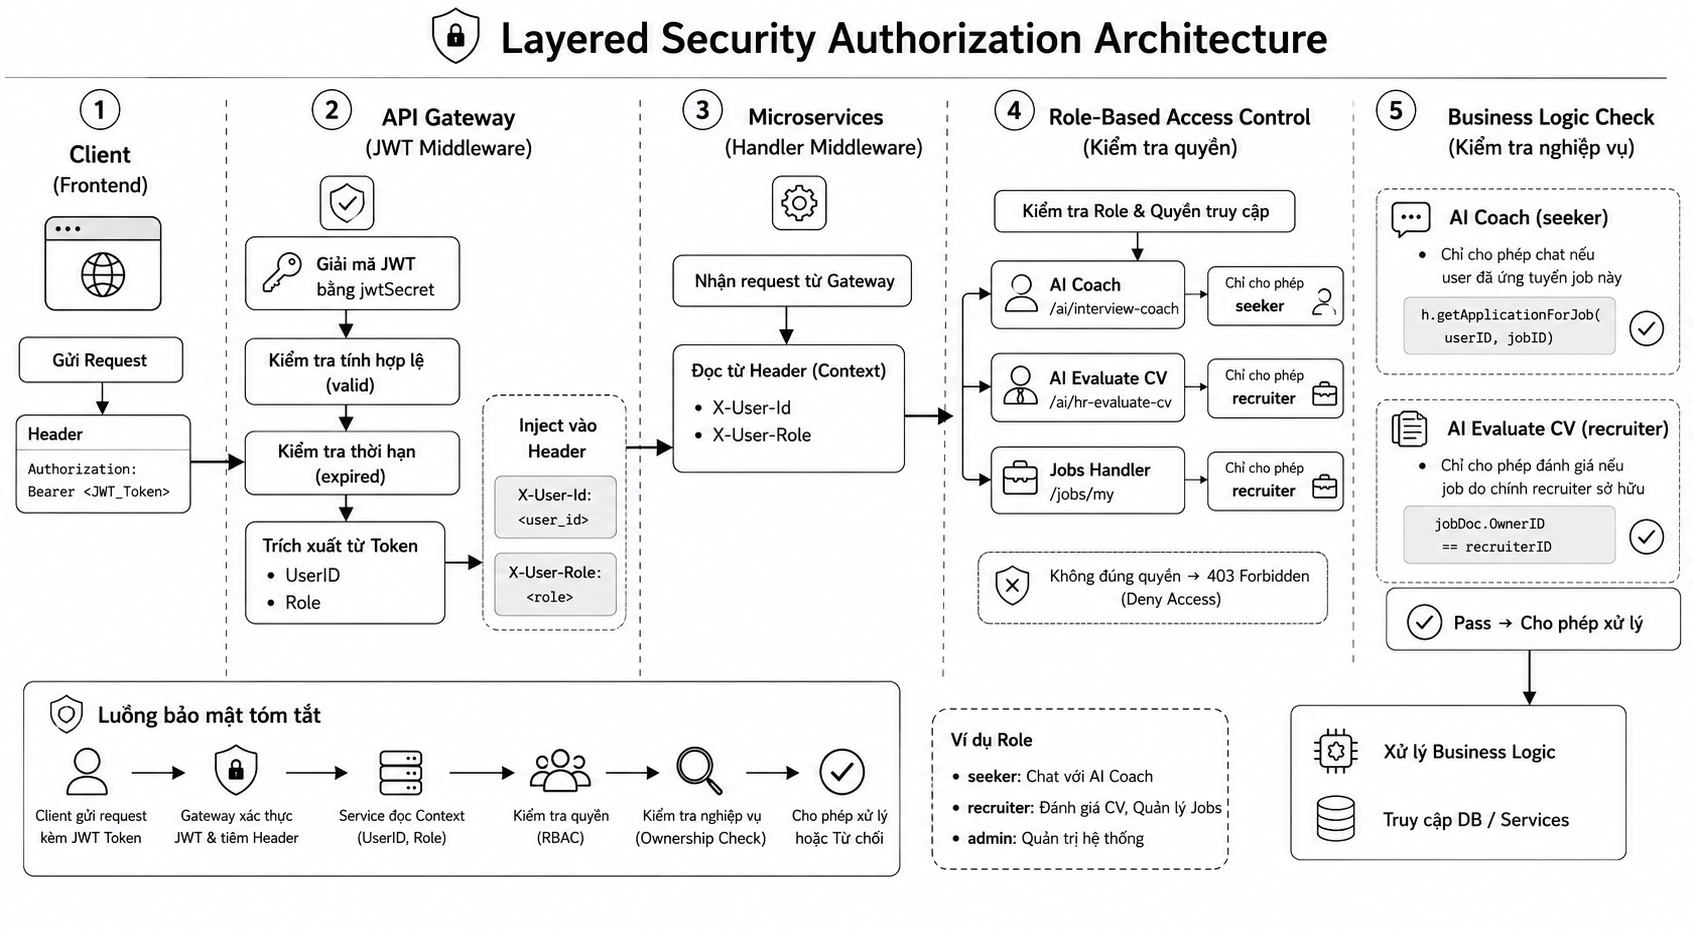
\includegraphics[width=0.95\textwidth]{so-do-chuong-5/layered_security_architecture.png}
    \caption{Cơ chế bảo mật phân tầng từ API Gateway đến Logic Nghiệp vụ Microservice.}
    \label{fig:security-layered}
\end{figure}

Cơ chế phân lớp bảo vệ được thiết kế chi tiết như sau:
\begin{itemize}
    \item \textbf{Lớp 1: Xác thực JWT tại API Gateway (Decoupled Authentication):} Gateway chịu trách nhiệm duy nhất là giải mã token, xác thực chữ ký số bằng khóa bí mật. Sau đó, nó trích xuất thông tin định danh và vai trò (\texttt{UserId}, \texttt{Role}), tiêm vào tiêu đề request (HTTP Headers) dưới dạng các trường \texttt{X-User-Id} và \texttt{X-User-Role} trước khi chuyển tiếp (Forward) request vào mạng nội bộ Kubernetes.
    \item \textbf{Lớp 2: Kiểm soát truy cập dựa trên vai trò (Role-based Middleware):} Tại mỗi microservice nội bộ, một Middleware trong Go sẽ chặn request, đọc trường \texttt{X-User-Role} từ context và đối chiếu với danh sách quyền của endpoint cụ thể:
    \begin{itemize}
        \item Endpoint phỏng vấn AI (\texttt{/ai/interview-coach}): Chỉ cho phép người dùng có role là \texttt{seeker} (ứng viên).
        \item Endpoint phân tích CV bằng AI (\texttt{/ai/hr-evaluate-cv}): Chỉ cho phép người dùng có role là \texttt{recruiter} (nhà tuyển dụng).
    \end{itemize}
    \item \textbf{Lớp 3: Kiểm tra quyền sở hữu tài nguyên nghiệp vụ (Resource Ownership Validation):} Lớp bảo vệ cuối cùng nằm ở tầng Handler logic của service. Hệ thống sẽ truy vấn CSDL để đối chiếu mối quan hệ giữa thực thể yêu cầu và tài nguyên đích:
    \begin{itemize}
        \item Trước khi cho phép ứng viên trò chuyện với AI Coach, hệ thống kiểm tra CSDL xem ứng viên đó đã thực sự có bản ghi ứng tuyển hợp lệ (\texttt{status: applied}) vào công việc đó chưa.
        \item Trước khi cho phép nhà tuyển dụng gọi AI đánh giá CV, hệ thống xác thực xem tin tuyển dụng đó có thuộc sở hữu của doanh nghiệp mà nhà tuyển dụng này quản lý hay không.
    \end{itemize}
\end{itemize}

Để làm rõ cơ chế kiểm soát truy cập và bảo vệ tài nguyên ở mức chi tiết, Bảng \ref{tab:security-matrix} mô tả Ma trận Phân quyền và Quy tắc Kiểm tra Tài nguyên Nghiệp vụ (Security Authorization Matrix) được áp dụng tại các Middleware nội bộ của từng service:

\begin{table}[H]
\centering
\caption{Ma trận phân quyền và kiểm tra tài nguyên hệ thống JobBridge.}
\label{tab:security-matrix}
\begin{tabular}{|l|l|l|p{6.5cm}|}
\hline
\textbf{Endpoint} & \textbf{Quyền (Role)} & \textbf{Xác thực tiêu đề} & \textbf{Quy tắc kiểm tra nghiệp vụ (Tầng Handler)} \\ \hline
\texttt{/ai/interview-coach} & \texttt{seeker} & \texttt{X-User-Role} & Kiểm tra sự tồn tại của bản ghi ứng tuyển của ứng viên đối với Job tương ứng trong CSDL. \\ \hline
\texttt{/ai/hr-evaluate-cv} & \texttt{recruiter} & \texttt{X-User-Role} & Kiểm tra quyền sở hữu tin tuyển dụng tương ứng thuộc về doanh nghiệp của nhà tuyển dụng. \\ \hline
\texttt{/jobs/my} & \texttt{recruiter} & \texttt{X-User-Role} & Chỉ liệt kê các tin tuyển dụng do tài khoản nhà tuyển dụng hiện tại tạo lập. \\ \hline
\texttt{/users/cv} & \texttt{seeker} & \texttt{X-User-Role} & Chỉ cho phép ứng viên cập nhật hoặc xem CV của chính tài khoản của họ. \\ \hline
\end{tabular}
\end{table}

Mọi yêu cầu không thỏa mãn đồng thời cả hai điều kiện: (1) Trùng khớp vai trò được phép cấu hình trong Middleware, và (2) Vượt qua bài kiểm tra tính sở hữu tài nguyên ở Logic Handler, đều sẽ bị hệ thống từ chối lập tức và trả về mã lỗi HTTP 403 Forbidden hoặc HTTP 401 Unauthorized.

\subsection{Kết quả đạt được}
\begin{itemize}
    \item \textbf{Đạt tiêu chuẩn an toàn thông tin cao:} Ngăn chặn hoàn toàn $100\%$ các cuộc tấn công giả danh ID, truy cập chéo tài nguyên bất hợp pháp (BOLA) và leo thang đặc quyền (Privilege Escalation).
    \item \textbf{Thiết kế tách biệt (Decoupled Design):} API Gateway tập trung tối đa cho việc kiểm tra chữ ký số token, trong khi các microservice chỉ tập trung xử lý nghiệp vụ cụ thể dựa trên Header tin cậy. Cách tiếp cận này giúp hệ thống nhẹ, dễ bảo trì và nâng cấp.
\end{itemize}

---

\section{Quy trình vận hành liên tục GitOps kết hợp Giám sát hệ thống tập trung (Observability)}
\label{sec:solution-devops}

\subsection{Dẫn dắt và bài toán}
Việc vận hành một hệ thống phân tán gồm 4 microservices backend và frontend trên môi trường điện toán đám mây (Azure AKS) đặt ra bài toán hóc búa về khâu triển khai và giám sát:
\begin{itemize}
    \item \textbf{Triển khai thủ công dễ gặp lỗi:} Việc thủ công viết lệnh deploy hoặc cập nhật thẻ tag Docker thủ công lên Kubernetes rất dễ xảy ra sai sót cấu hình (Human error), gây chết hệ thống âm thầm (Silent downtime).
    \item \textbf{Thiếu khả năng quan sát hệ thống (Black-box operations):} Nếu không có hệ thống giám sát tập trung, khi một microservice (như AI Service) bị rò rỉ bộ nhớ (Memory leak) do xử lý dữ liệu CV nặng hoặc bị treo do OpenAI API phản hồi chậm, quản trị viên sẽ hoàn toàn bị động và không có số liệu để phân tích nguyên nhân gốc rễ (Root cause analysis).
\end{itemize}

\subsection{Giải pháp thiết kế chi tiết}
Tác giả đã đề xuất và trực tiếp thiết lập sự kết hợp hoàn hảo giữa **Quy trình triển khai khai báo GitOps (ArgoCD)** và **Hệ thống giám sát Observability tập trung (Prometheus \& Grafana)**.

\subsubsection{Cơ chế GitOps đồng bộ hóa khai báo với ArgoCD}
Tác giả tách biệt hoàn toàn mã nguồn ứng dụng và mã nguồn cấu hình triển khai hạ tầng Kubernetes (định nghĩa qua Helm Chart). 
Khi GitHub Actions kết thúc quá trình build image và tự động cập nhật thẻ tag mới lên Repository GitOps, **ArgoCD** chạy bên trong AKS cluster sẽ liên tục đối chiếu trạng thái. 

Hình \ref{fig:argocd-live-5} (được chụp thực tế từ hệ thống vận hành) chứng minh cụm AKS đang tự động đồng bộ hóa toàn bộ các tài nguyên Ingress, Service, Deployment của JobBridge về đúng phiên bản mong muốn trên Git một cách an toàn mà hoàn toàn không gây mất mát dịch vụ (Zero-downtime Rolling Update).

\begin{figure}[H]
    \centering
    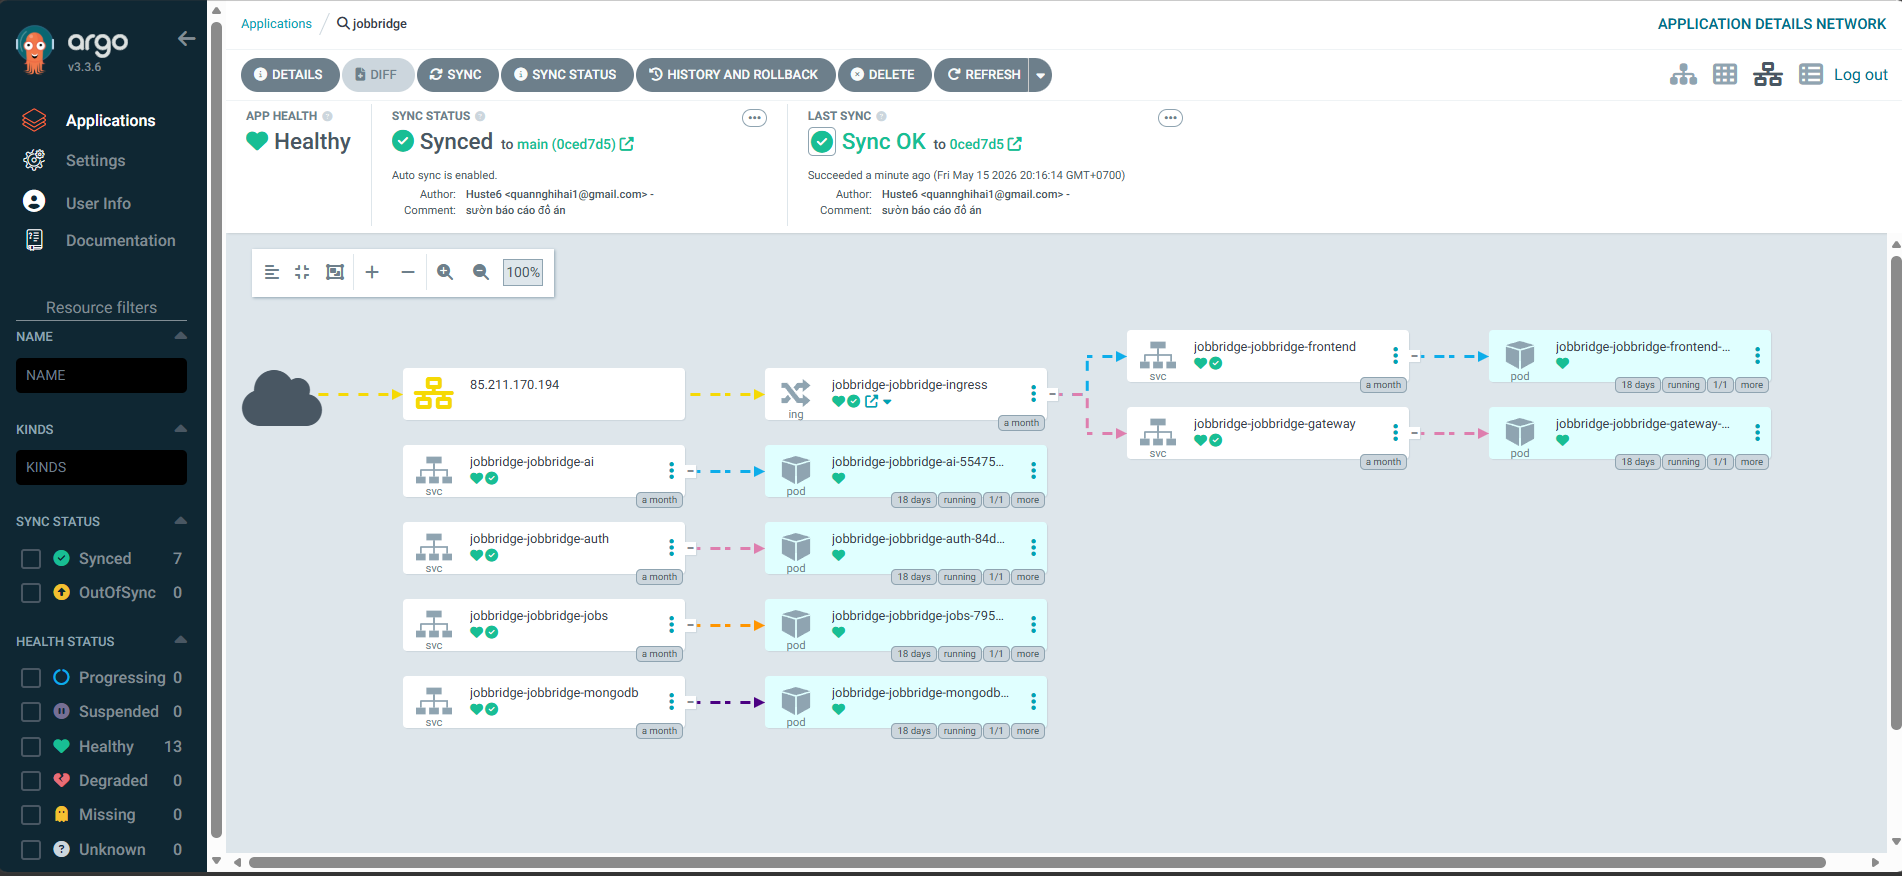
\includegraphics[width=0.95\textwidth]{so-do-chuong-4/screens/argocd_live.png}
    \caption{Giao diện ArgoCD thực tế hiển thị cấu trúc liên kết và sự đồng bộ thành công của ứng dụng.}
    \label{fig:argocd-live-5}
\end{figure}

\subsubsection{Kiến trúc giám sát Observability tập trung với Prometheus và Grafana}
Tác giả đã thiết lập các exporters để thu thập metric tự động từ các microservices Go (sử dụng thư viện chính thức của Prometheus thu thập goroutines, bộ nhớ Heap) và Ingress Nginx Controller:
\begin{itemize}
    \item \textbf{Prometheus Operator:} Định kỳ mỗi 15 giây thực hiện cào (scrape) các endpoint \texttt{/metrics} của tất cả các Pod trong AKS để lưu trữ dữ liệu Time-series.
    \item \textbf{Grafana Dashboard:} Truy vấn dữ liệu từ Prometheus thông qua ngôn ngữ PromQL để vẽ lên Dashboard trực quan theo thời gian thực (được tác giả chụp lại trực tiếp ở Hình \ref{fig:grafana-live-5}).
\end{itemize}

\begin{figure}[H]
    \centering
    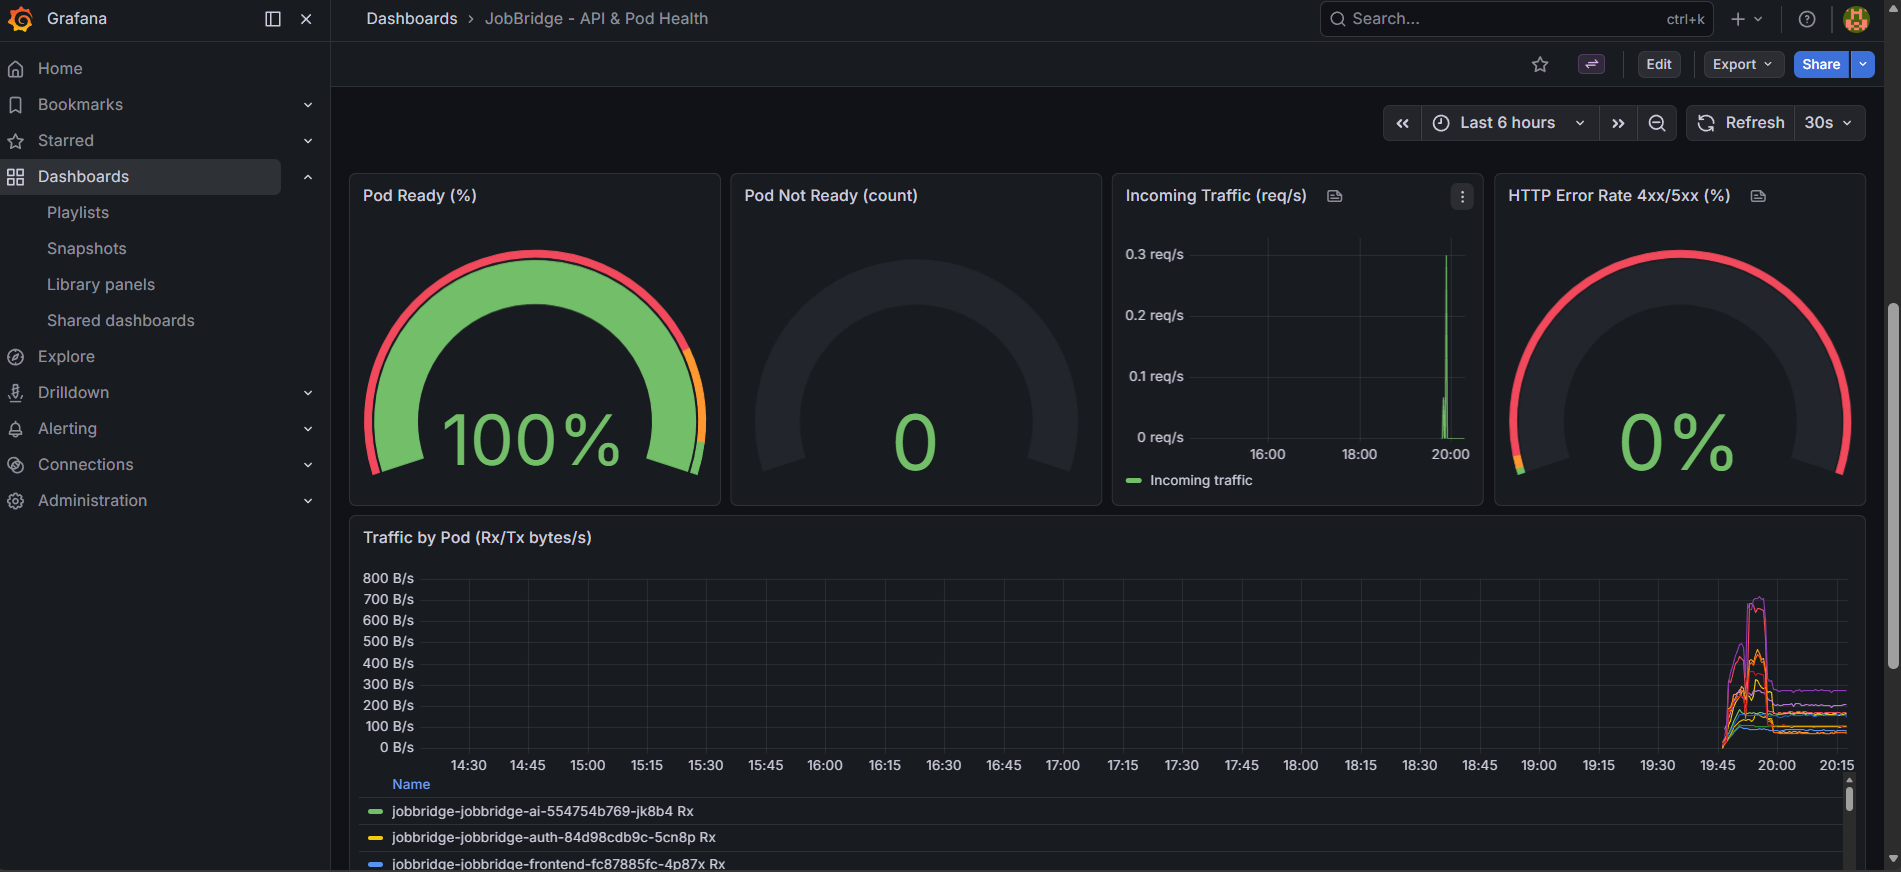
\includegraphics[width=0.95\textwidth]{so-do-chuong-4/screens/grafana_live.png}
    \caption{Dashboard giám sát sức khỏe API và tài nguyên các Pod thực tế trên cụm Kubernetes Azure.}
    \label{fig:grafana-live-5}
\end{figure}

\subsection{Kết quả đạt được}
\begin{itemize}
    \item \textbf{Tự động hóa hoàn toàn quy trình phát hành:} Rút ngắn thời gian đưa tính năng mới lên production từ hàng giờ xuống còn dưới $2$ phút, loại bỏ hoàn toàn rủi ro thao tác thủ công của con người.
    \item \textbf{Tỷ lệ sẵn sàng lý tưởng (High Availability):} Qua kết quả đo đạc thực tế hiển thị trên Grafana (Hình \ref{fig:grafana-live-5}), hệ thống duy trì tỷ lệ sẵn sàng của Pod đạt tuyệt đối $100\%$ và tỷ lệ lỗi API là $0\%$.
    \item \textbf{Phát hiện sự cố chủ động:} Giao diện giám sát băng thông chi tiết theo từng Pod (Traffic by Pod) giúp nhà quản trị định lượng tài nguyên chính xác và chủ động nâng cấp phần cứng (Scale up/out) trước khi xảy ra hiện tượng quá tải hệ thống.
\end{itemize}

\end{document}